\documentclass{article}
\usepackage{longtable}
\usepackage{graphicx}
\usepackage{bm}
\usepackage{aligned-overset}
\usepackage[slantfont,boldfont]{xeCJK}
\usepackage{fontspec}
\setCJKmainfont{SimSun}
\setmainfont{SimSun}
\setsansfont{SimSun}

\title{谐振电路实验报告}
\author{2411545 邱凯锐}
\date{2025.3.3}

\begin{document}
\maketitle
\section{实验目的}
\hspace*{2em}(1)了解RLC组合交流电路的阻抗对频率的依赖关系。\\
\hspace*{2em}(2)掌握谐振电路的谐振条件及谐振特点。\\
\hspace*{2em}(3)了解谐振曲线的形状与线路Q值的关系。

\section{实验仪器}
\hspace*{2em}(1)信号源:F05型数字合成函数/任意波信号发生器/计数器\\
\hspace*{2em}(2)示波器:OWON XDS3102A\\
\hspace*{2em}(3) 7X28A/10型交流/直流电阻箱 $\times 2$\\
\hspace*{2em}(4) BR8/3型标准电容器 $0.1\mu F$(中华人民共和国上海沪光仪器厂)\\
\hspace*{2em}(5) 电感线圈 $0.1H$

\section{实验原理}
\begin{figure}[!h]
    \centering
    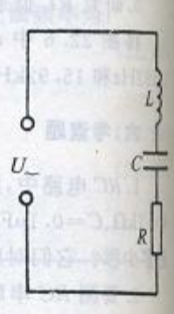
\includegraphics[width=2cm]{3.png}
    \caption{$RLC$串联电路}
    \end{figure}
\hspace*{2em}$RCL$串联电路的复阻抗为:
$$
\bm{Z}=\bm{Z_R}+\bm{Z_L}+\bm{Z_C} =R+\textup{j}(\omega L-\frac{1}{\omega C})
$$
复阻抗的模:
$$
Z=\sqrt{R^2+(\omega L-\frac{1}{\omega C})^2}
$$
复阻抗的幅角:
$$
\varphi=\arctan\frac{\omega L-\frac{1}{\omega C}}{R}
$$
$\varphi$角即该电路电流滞后与总电压的相位差。回路中电流$I$(有效值)为:
$$
I=\frac{U}{\sqrt{R^2+(\omega L-\frac{1}{\omega C})^2}}
$$
\hspace*{2em} 改变电源频率,当$\omega L-\frac{1}{\omega C}=0$时,$\varphi=0$,表明电路中电流$I$和电压$U$同位相,整个电路呈现纯电阻性,这就是串联谐振现象。此时电路总阻抗的模$Z=R$为最小,如$U$不随$f$变化,电流$I$则达到极大值。
\\
\hspace*{2em}令$\omega_0$和$f_0$表示谐振状态下的圆频率和频率,由谐振条件$\omega L-\frac{1}{\omega C}$可得:
$$
\omega_0=\sqrt{\frac{1}{LC}}\quad 或 \quad{f_0}=\frac{\omega_0}{2\pi}
$$
$R、L、C$元件上的电压有效值分别为:
\begin{equation}
\begin{aligned}
    &U_R=IR=\frac{R}{\sqrt{R^2+(\omega L-\frac{1}{\omega C})^2}}U \\
    &U_L=I\omega L=\frac{\omega L}{\sqrt{R^2+(\omega L-\frac{1}{\omega C})^2}}U  \\
    &U_L=I\omega L=\frac{1}{\omega C\sqrt{R^2+(\omega L-\frac{1}{\omega C})^2}}U 
\end{aligned}
\end{equation}

\hspace*{2em} 电路发生谐振时,(1)式变为:
\begin{equation}
    \begin{aligned}
        &U_R=U \\
        &U_L=\frac{\omega_0 L}{R}U=QU  \\
        &U_L=\frac{1}{\omega_0RC}U=QU
    \end{aligned}
    \end{equation}
式中\hspace*{2em} $Q=\frac{\omega_0L}{R}=\frac{1}{R}\sqrt{\frac{L}{C}}$\\
称$Q$为串联谐振电路的品质因数,R为串联谐振电路的总电阻。\\
\hspace*{2em}同时对于$I-f$曲线,通常考查$I$由极大值$I_{max}$下降到$I_{max}/\sqrt{2}=0.707I_{max}$时的两点对应频率$f_1$和$f_2$之差$\Delta f$($\Delta f=f_2-f_1$称为通频带宽度)与谐振频率$f_0$的关系,可以证明它们之间的关系满足下式:
$$
\frac{\Delta f}{f_0}=\frac{1}{Q}
$$
\section{实验内容}
\hspace*{2em}按电路图联结电路。\\
\hspace*{2em}(1) $R$置$100\Omega $,置$R'+R_L=100\Omega$($R_L$为$L$串联损耗电阻,本实验中$R_L=13\Omega$),保持$U=3.00V$不变,用示波器测出不同频率$f$下的$U_R$,从而作出$I-f$关系曲线,并在谐振频率下测出$U_L$和$U_C$值;由示波器测出$\varphi -f$关系曲线。\\
\hspace*{2em}(2) $R$置$100\Omega $,置$R'+R_L=300\Omega$,仍保持$U=3.00V$不变,测出$I-f$曲线,谐振频率下的$U_L$和$U_C$值,以及$\varphi -f$关系曲线。\\
\hspace*{2em}从上诉曲线上找出谐振频率的测量值$f_{0测}$,由谐振时测得的$U_C$(或者$U_L$)值求出$Q_{串测}$。将$f_{0测}$和$Q_{串测}$与理论值$f_{0测}$和$Q_{串理}$相比较。\\
\hspace*{2em} 在两条曲线上,找到谐振峰两旁的$I_{max}/\sqrt{2}$值所相应的频率$f_1$和$f_2$,算出$Q$值,并于理论值比较。

\begin{figure}[!h]
    \centering
    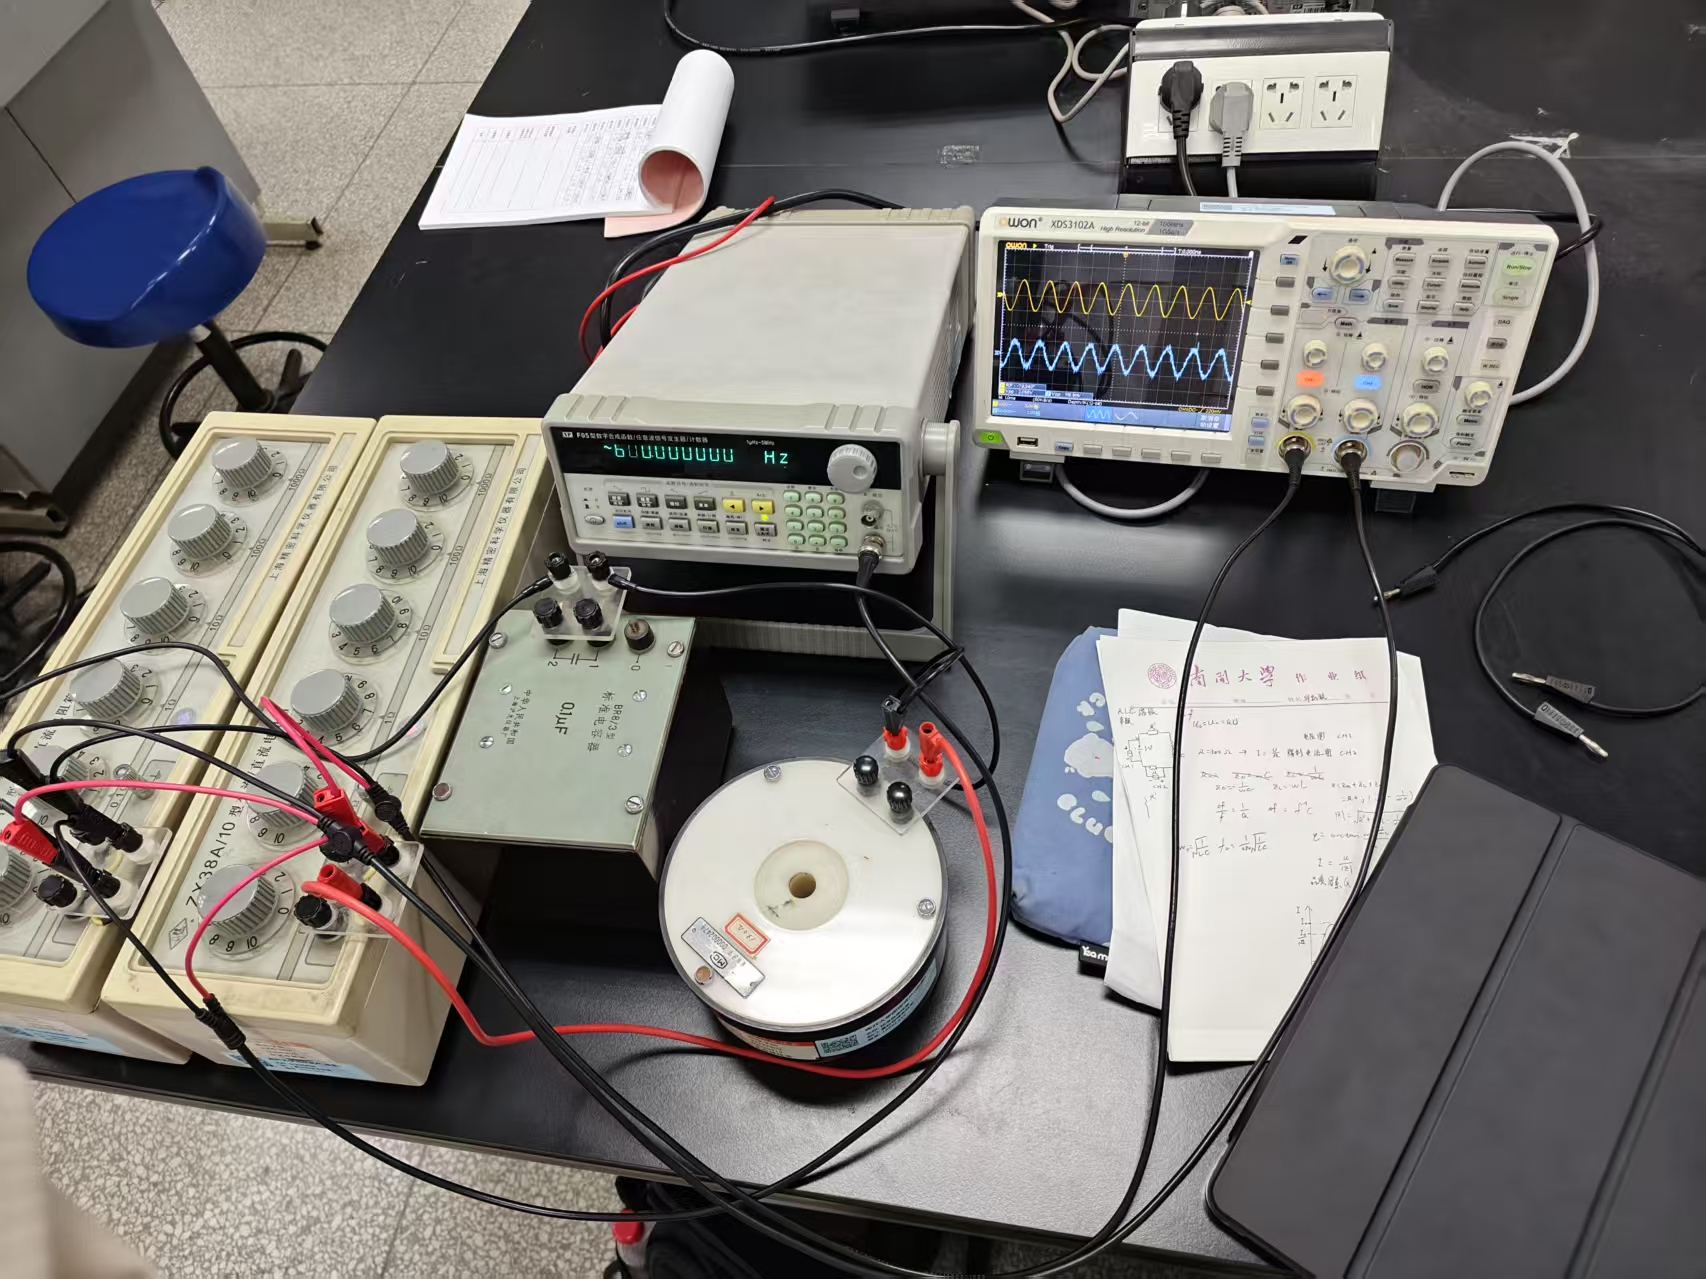
\includegraphics[width=9cm]{123.jpg}
    \caption{实验装置}
\end{figure}

\section{实验数据}

\begin{longtable}{ccccc}
    % \centering
    \caption[Short Caption]{$R'+R_L=100\Omega$}
    \label{table:longtable_example} \\
    
    % 下面是表头
    \hline  频率(Hz) & 电压U(V) & 电流I(mA) & 相位$\varphi$(角度值) & (弧度制) \\ \hline 
    \endfirsthead
    
    % 下面数字3的意思是表格的列数
    \multicolumn{5}{c}%
    {{\bfseries \tablename\ \thetable{} -- continued from previous page}} \\
    \hline 频率(Hz) & 电压U(V) & 电流I(mA) & 相位$\varphi$(角度值) & (弧度制) \\  \hline  
    % 注意这里把表头复制了一遍,因为在新的页面也会展示一下表头,不然表格不方便阅读
    \endhead
    
    \hline \multicolumn{5}{r}{{Continued on next page}} \\ \hline
    \endfoot
    
    \hline \hline
    \endlastfoot
    600    & 123    & 1.23    & -89 & -1.553297222 \\ \hline
800    & 204    & 2.04    & -83 & -1.448580556 \\ \hline
1000   & 307    & 3.07    & -78 & -1.361316667 \\ \hline
1200   & 501    & 5.01    & -71 & -1.239147222 \\ \hline
1400   & 937    & 9.37    & -51 & -0.890091667 \\ \hline
1500   & 1260   & 12.6    & -30 & -0.523583333 \\ \hline
1550   & 1400   & 14      & -14 & -0.244338889 \\ \hline
1570   & 1440   & 14.4    & -7  & -0.122169444 \\ \hline
1590   & 1460   & 14.6    & -1  & -0.017452778 \\ \hline
1610   & 1450   & 14.5    & 6   & 0.104716667  \\ \hline
1630   & 1420   & 14.2    & 12  & 0.209433333  \\ \hline
1650   & 1370   & 13.7    & 19  & 0.331602778  \\ \hline
1700   & 1220   & 12.2    & 32  & 0.558488889  \\ \hline
1900   & 717    & 7.17    & 59  & 1.029713889  \\ \hline
2100   & 508    & 5.08    & 69  & 1.204241667  \\ \hline
2300   & 383    & 3.83    & 75  & 1.308958333  \\ \hline
2500   & 309    & 3.09    & 79  & 1.378769444  \\ \hline
2700   & 270    & 2.7     & 80  & 1.396222222  \\ \hline
    \end{longtable}

\begin{longtable}{ccccc}
    % \centering
    \caption[Short Caption]{$R'+R_L=300\Omega$}
    \label{table:longtable_example} \\
    
    % 下面是表头
    \hline  频率(Hz) & 电压U(V) & 电流I(mA) & 相位$\varphi$(角度值) & (弧度制) \\ \hline 
    \endfirsthead
    
    % 下面数字3的意思是表格的列数
    \multicolumn{5}{c}%
    {{\bfseries \tablename\ \thetable{} -- continued from previous page}} \\
    \hline 频率(Hz) & 电压U(V) & 电流I(mA) & 相位$\varphi$(角度值) & (弧度制) \\  \hline  
    % 注意这里把表头复制了一遍,因为在新的页面也会展示一下表头,不然表格不方便阅读
    \endhead
    
    \hline \multicolumn{5}{r}{{Continued on next page}} \\ \hline
    \endfoot
    
    \hline \hline
    \endlastfoot
    600    & 127    & 1.27    & -79 & -1.378769444 \\ \hline
800    & 197    & 1.97    & -76 & -1.326411111 \\ \hline
1000   & 285    & 2.85    & -68 & -1.186788889 \\ \hline
1200   & 432    & 4.32    & -56 & -0.977355556 \\ \hline
1400   & 622    & 6.22    & -33 & -0.575941667 \\ \hline
1500   & 712    & 7.12    & -16 & -0.279244444 \\ \hline
1550   & 733    & 7.33    & -5  & -0.087263889 \\ \hline
1570   & 738    & 7.38    & -3  & -0.052358333 \\ \hline
1590   & 740    & 7.4     & 0   & 0            \\ \hline
1610   & 739    & 7.39    & 3   & 0.052358333  \\ \hline
1630   & 735    & 7.35    & 4   & 0.069811111  \\ \hline
1650   & 728    & 7.28    & 11  & 0.191980556  \\ \hline
1700   & 703    & 7.03    & 18  & 0.31415      \\ \hline
1900   & 553    & 5.53    & 40  & 0.698111111  \\ \hline
2100   & 437    & 4.37    & 52  & 0.907544444  \\ \hline
2300   & 351    & 3.51    & 61  & 1.064619444  \\ \hline
2500   & 293    & 2.93    & 66  & 1.151883333  \\ \hline
2700   & 258    & 2.58    & 70  & 1.221694444  \\ \hline
    \end{longtable}

    \begin{longtable}{ccc}
        % \centering
        \caption[Short Caption]{谐振频率下$U_C$和$U_L$的值}
        \label{table:longtable_example} \\
        
        % 下面是表头
        \hline  组别 & $U_C(V)$ & $U_L(V)$ \\ \hline 
        \endfirsthead
        
        % 下面数字3的意思是表格的列数
        \multicolumn{3}{c}%
        {{\bfseries \tablename\ \thetable{} -- continued from previous page}} \\
        \hline 组别 & $U_C(V)$ & $U_L(V)$ \\  \hline  
        % 注意这里把表头复制了一遍,因为在新的页面也会展示一下表头,不然表格不方便阅读
        \endhead
        
        \hline \multicolumn{3}{r}{{Continued on next page}} \\ \hline
        \endfoot
        
        \hline \hline
        \endlastfoot
        1 & 14.3 & 14.4\\ \hline
        2 & 7.2  & 7.2\\ \hline
       
        \end{longtable}
\begin{figure}[!h]
    \centering
    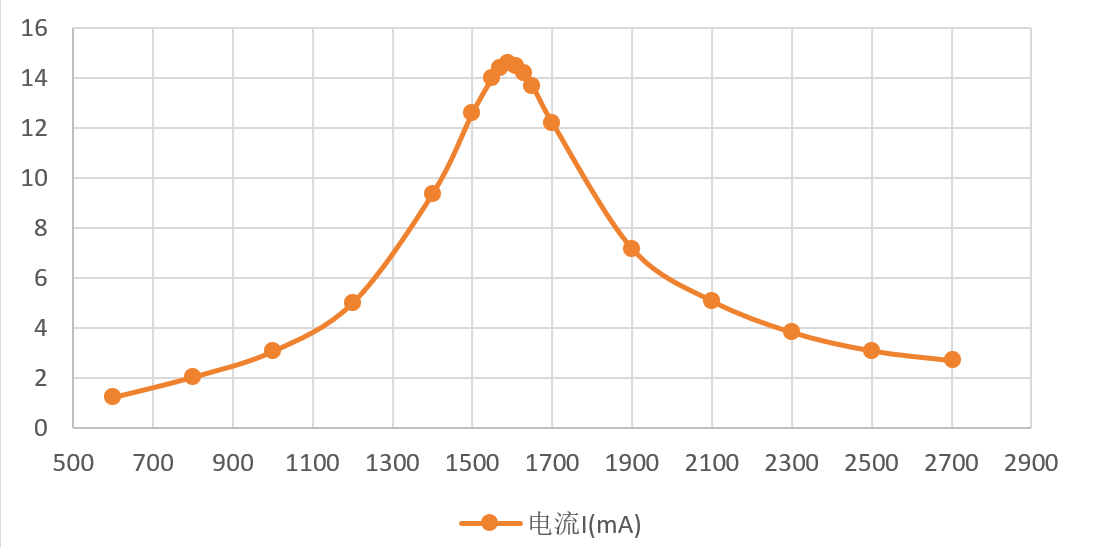
\includegraphics[width=9cm]{11.png}
    \caption{$I-f$曲线($R'+R_L=100\Omega$)}
    \end{figure}
\begin{figure}[!h]
    \centering
    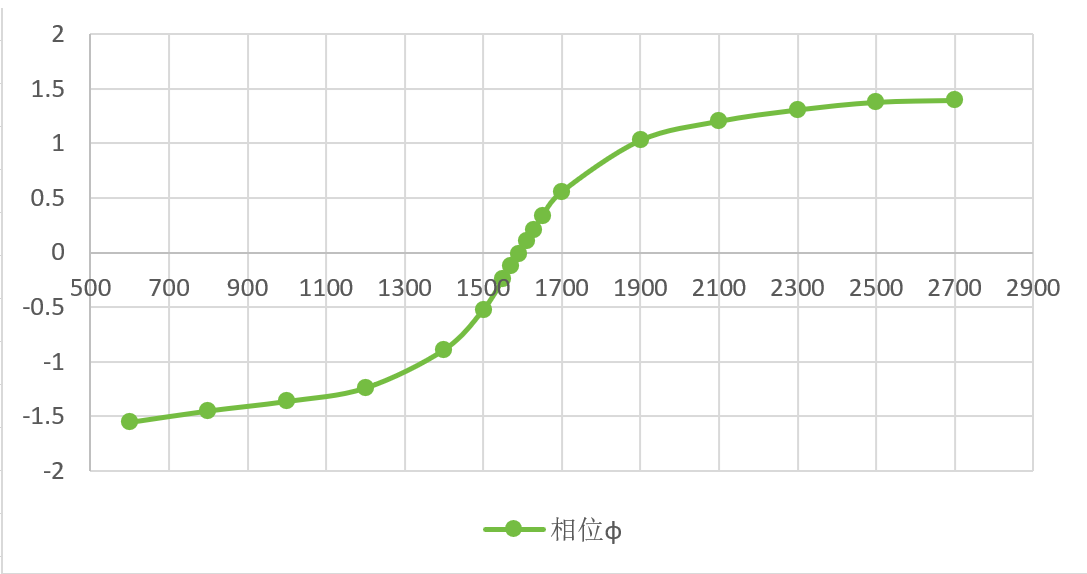
\includegraphics[width=9cm]{12.png}
    \caption{$\varphi-f$曲线($R'+R_L=100\Omega$)}
    \end{figure}
\begin{figure}[!h]
    \centering
    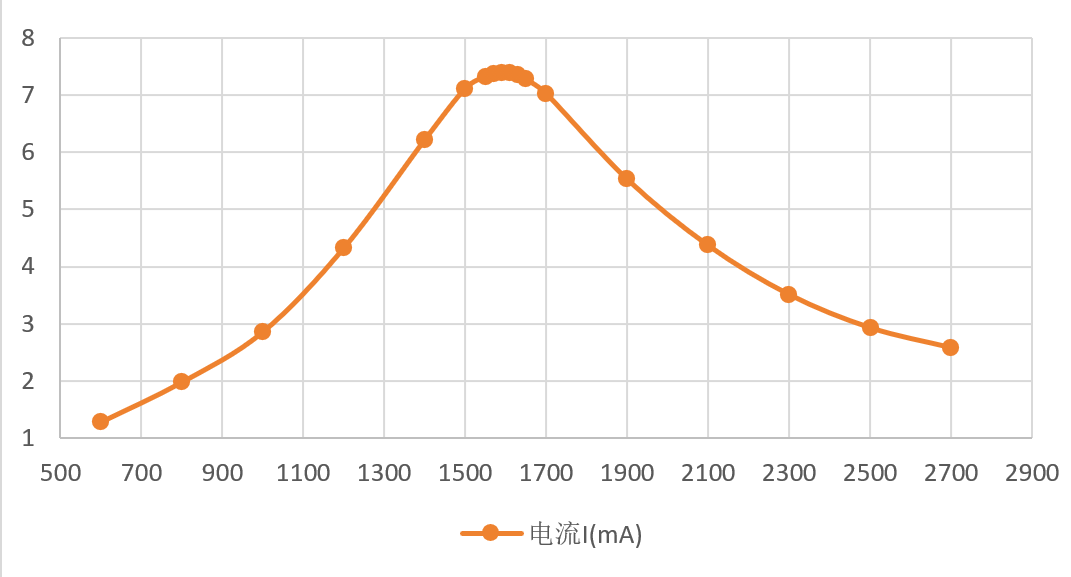
\includegraphics[width=9cm]{21.png}
    \caption{$I-f$曲线($R'+R_L=300\Omega$)}
\end{figure}
\begin{figure}[!h]
    \centering
    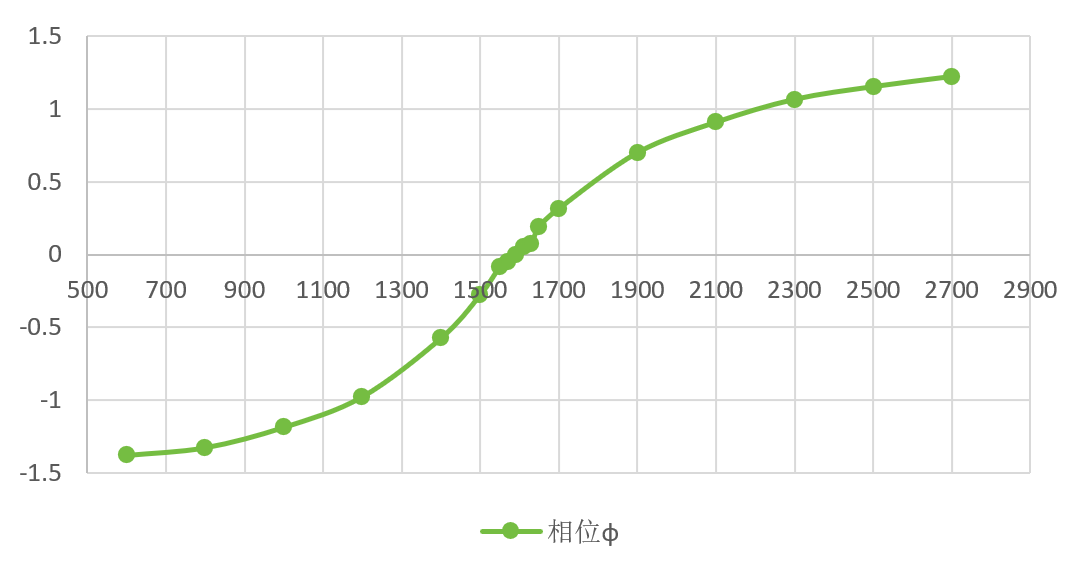
\includegraphics[width=9cm]{22.png}
    \caption{$\varphi-f$曲线($R'+R_L=300\Omega$)}
\end{figure}

\begin{longtable}{ccccc}
    % \centering
    \caption[Short Caption]{$f(KHz)$值比较}
    \label{table:longtable_example} \\
    
    % 下面是表头
    \hline  组别 & $f_{0理}$ & $f_{0测}$ & $f_1$ & $f_2$\\ \hline 
    \endfirsthead
    
    % 下面数字3的意思是表格的列数
    \multicolumn{5}{c}%
    {{\bfseries \tablename\ \thetable{} -- continued from previous page}} \\
    \hline 组别 & $f_{0理}$ & $f_{0测}$ & $f_1$ & $f_2$\\  \hline  
    % 注意这里把表头复制了一遍,因为在新的页面也会展示一下表头,不然表格不方便阅读
    \endhead
    
    \hline \multicolumn{5}{r}{{Continued on next page}} \\ \hline
    \endfoot
    
    \hline \hline
    \endlastfoot
    1 & 1.59 & 1.58 & 1.43  & 1.76\\ \hline
    2 & 1.59  & 1.59 &1.30 &1.95\\ \hline
   
    \end{longtable}

\begin{longtable}{ccccc}
    % \centering
    \caption[Short Caption]{$Q$值比较}
    \label{table:longtable_example} \\
    
    % 下面是表头
    \hline  组别 & $Q_{串理}$ & $Q_{串测1}=\frac{U_C}{U}$ &$Q_{串测2}=\frac{f_0}{\Delta f}$\\ \hline 
    \endfirsthead
    
    % 下面数字3的意思是表格的列数
    \multicolumn{4}{c}%
    {{\bfseries \tablename\ \thetable{} -- continued from previous page}} \\
    \hline  组别 & $Q_{串理}$ & $Q_{串测1}$  & $Q_{串测2}=\frac{f_0}{\Delta f}$\\  \hline  
    % 注意这里把表头复制了一遍,因为在新的页面也会展示一下表头,不然表格不方便阅读
    \endhead
    
    \hline \multicolumn{4}{r}{{Continued on next page}} \\ \hline
    \endfoot
    
    \hline \hline
    \endlastfoot
    1 & 4.99 & 4.81 & 4.82\\ \hline
    2 & 2.50  & 2.41 & 2.45\\ \hline
   
    \end{longtable}

\section{总结}
\hspace*{2em}本次实验较为成功地完成了实验目标,成功测出$I-f$以及$\varphi-f$曲线,谐振频率$f_0$和品质因数$Q$的测量值与理论值也较为接近。
\\
\hspace*{2em}同时通过本次实验,我对示波器、信号源等电路设备的使用有了初步的认识,了解了相关的使用事项,为日后的实验课打好了基础。

\end{document}